\documentclass[20pt,margin=2.2cm,innermargin=-4.5in,blockverticalspace=-0.25in]{tikzposter}

\geometry{paperwidth=80cm,paperheight=120cm} %A0
% \geometry{paperheight=33.11in,paperwidth=23.4in} %A1
\usepackage[utf8]{inputenc}
\usepackage[spanish]{babel}
\usepackage{amsmath}
\usepackage{amsfonts}
\usepackage{amsthm}
\usepackage{amssymb}
\usepackage{mathrsfs}
\usepackage{graphicx}
\usepackage{lipsum}
\usepackage[export]{adjustbox}
\usepackage{enumitem}
\usepackage[backend=biber,style=numeric]{biblatex}
\usepackage{ubtheme}
\makeatletter
\setlength{\TP@visibletextwidth}{75cm}
\setlength{ \TP@visibletextheight}{45in}
\makeatother
\usepackage{mwe} % for placeholder images
\usepackage{bm}
\usepackage{bbm}
\definecolor{bristolred}{HTML}{B01C2E}
\addbibresource{refs.bib}

% set theme parameters
\tikzposterlatexaffectionproofoff
\usetheme{UBTheme}
\usecolorstyle{UBStyle}
\useinnerblockstyle{Heldert}
\def \SL{SL_2(\mathbb{Z})}
\def\H{{ \!\! \rm \ I\!H}}
\newcommand{\set}[1]{ \left\{ #1 \right\} }

\makeatletter
\newcounter{tablecounter}
\newenvironment{tikztable}[1][]{
  \def \rememberparameter{#1}
  \vspace{10pt}
  \refstepcounter{tablecounter}
  \begin{center}
  }{
    \ifx\rememberparameter\@empty
    \else
    \\[10pt]
    {\small Tab.~\thetablecounter: \rememberparameter}
    \fi
  \end{center}
}
\makeatother

\usepackage[scaled]{helvet}
\renewcommand\familydefault{\sfdefault} 
\renewcommand{\vec}[1]{\bm{#1}}
\newcommand{\Tr}{\text{Tr}}
\usepackage[T1]{fontenc}

\title{\parbox{0.95\linewidth}{Una antolog\'ia de la obra de Conway}}
\author{\textbf{Roger David Trujillo Ib\'a\~nez}\textsuperscript{1}}
\institute{\textsuperscript{1}Departamento de Matemáticas, Universidad Nacional de Colombia}

\titlegraphic{
\includegraphics[width=0.23\textwidth]{Imagenes/PNG_LOGOSIMBOLO_LATERAL_NEGRO-02.png}}

% begin document
\begin{document}
\maketitle
\begin{columns}
    \column{0.5}
    \block{Descripción General}{
        John Conway naci\'o el 26 de diciembre de 1937, en Liverpool, Inglaterra. En los a\~nos 1970 se di\'o a conocer en la comunidad de matem\'aticas puras al encontrar tres grupos simples que nunca antes se hab\'ian encontrado, a estos ahora se les conoce por el nombre de \textit{Conway groups}, sin embargo, para la comunidad general de gente interesada en matem\'atica sus aportes m\'as destacables no fueron esos.

        Este trabajo se concentra en sus aportes a la matem\'atica recreativa, explicamos la historia de los conceptos, de d\'onde surgieron y hacemos una explicaci\'on matem\'atica.
        
        Explicamos tres trabajos de Conway: el juego de la vida, la teor\'ia de juegos combinatorios, y los n\'umeros surreales. Los dos primeros los abordamos divulgativamente, mientras que a los n\'umeros surreales le hacemos una descripci\'on formal, los definimos formalmente y demostramos que forman un cuerpo ordenado.

        Para la parte hist\'orica nos basamos fuertemente en su biograf\'ia, \textit{Genius at Play} \cite{Roberts2015-ur}.
    }
    

    
    \block{El juego de la vida}{
        Conway cuenta que fueron las ideas de c\'omo los aut\'omatas podr\'ian en alg\'un momento simular cosas complejas como el cerebro humano, o incluso, podr\'ian replicarse a s\'i mismas, las que dieron inicio a su inter\'es en crear aut\'omatas. Conway empez\'o a buscar automatas universales que tuvieran reglas simples, en esta b\'usqueda Conway cre\'o y estudi\'o varios aut\'omatas, FRACTRAN fue el primer resultado.
        \vspace{7mm}
        
        \innerblock{FRACTRAN}{
            Es un lenguaje de programaci\'on cuyos programas consisten en una lista finitas de fracciones. FRACTRAN puede crear cualquier programa posible, por ejemplo, este es un programa que genera los n\'umeros primos en orden
            \[
                {\displaystyle \left({\frac {17}{91}},{\frac {78}{85}},{\frac {19}{51}},{\frac {23}{38}},{\frac {29}{33}},{\frac {77}{29}},{\frac {95}{23}},{\frac {77}{19}},{\frac {1}{17}},{\frac {11}{13}},{\frac {13}{11}},{\frac {15}{14}},{\frac {15}{2}},{\frac {55}{1}}\right)}.
            \]

        }

        \vspace{5mm}
        Luego de esto Conway empez\'o a estudiar aut\'omatas celulares de dos dimensiones, inspirado en las idead de Von Neumann.

        El juego de la vida se juega en un tablero dos dimensional conformado por celdas, como un tablero de Go pero infinito. El juego empieza con un estado inicial y va evolucionando conforme a las reglas. Cada celda tiene 8 celdas adyacentes a los que llamaremos vecinos, cuatro que comparten un lado y cuatro que comparten solamente un v\'ertice, es decir, dos horizontales, dos verticales, y cuatro en diagonal. Las reglas del juego son:
        \vspace{7mm}
        
        \innerblock{Reglas}{
            \begin{enumerate}
                \item \textbf{Regla de nacimiento:} Si una celda est\'a muerta en el tiempo $t$, y la celda tiene exactamente $3$ celdas vecinas que est\'an vivas, entonces la celda se convierte en una celda viva en el tiempo $t+1$.
                \item \textbf{Regla de muerte:} Si una celda viva en el tiempo $t$ tiene menos que $2$ vecinos vivos, la celda muere por soledad en el tiempo $t+1$. Si una celda viva en el tiempo $t$ tiene m\'as que $3$ vecinos vivos, la celda muere por hacinamiento en el tiempo $t+1$.
                \item \textbf{Regla de supervivencia:} Si una celda viva tiene exactamente $2$ o $3$ celdas vivas vecinas, entonces la celda sigue viva en el tiempo $t+1$.
            \end{enumerate}

        }

        \vspace{5mm}
        La figura más importante que se descubri\'o al comienzo del estudio del juego de la vida fue el \textit{glider}, un patr\'on que pod\'ia ``moverse'' por el tablero. El \textit{glider} era importante porque permit\'ia mandar informaci\'on por el tablero, cuando Conway y su equipo encontraron el \textit{glider} se imaginaron que podr\'ia funcionar como la corriente el\'ectrica funciona en los computadores, enviando se\~nales.
        \vspace{7mm}

        \begin{minipage}[t]{\linewidth}
            \centering
            \begin{minipage}[t]{0.15\linewidth}
                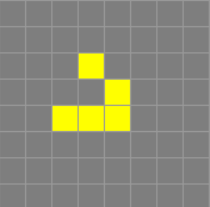
\includegraphics[width=\textwidth]{images/life-glider-1.png}
            \end{minipage}
            \begin{minipage}[t]{0.15\linewidth}
                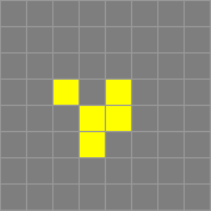
\includegraphics[width=\textwidth]{images/life-glider-2.png}
            \end{minipage}
            \begin{minipage}[t]{0.15\linewidth}
                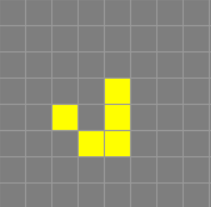
\includegraphics[width=\textwidth]{images/life-glider-3.png}
            \end{minipage}
            \begin{minipage}[t]{0.15\linewidth}
                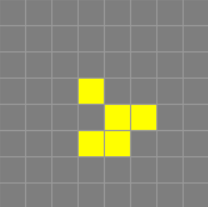
\includegraphics[width=\textwidth]{images/life-glider-4.png}
            \end{minipage}
            \begin{minipage}[t]{0.15\linewidth}
                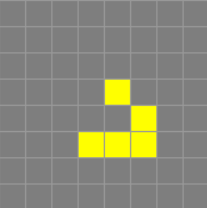
\includegraphics[width=\textwidth]{images/life-glider-5.png}
            \end{minipage}
        \end{minipage}

        \vspace{5mm}
        En Octubre de 1970, Martin Gardner en su columna \textit{Mathematical Games} del \textit{Scientific American} \cite{Gardner1970} escribi\'o un texto titulado \textit{The fantastic combinations of John Conway's new solitaire game ``life''}. La columna, adem\'as de describir el juego propon\'ia un reto; encontrar un patr\'on inicial que al evolucionar creciera sin l\'imites, y adem\'as promet\'ia 50 USD a quien fuera el primero en encontrarla o demostrar que no existe.

        En Noviembre del a\~no en que sali\'o la columna de Gardner (1970), un equipo del MIT liderado por Bill Gosper, un matem\'atico y programador estadounidense, se gan\'o el premio propuesto en la columna al descubrir/inventar una pistola de gliders ahora conocida como la \textit{Gosper Glider gun}
        \vspace{7mm}

        \begin{minipage}[t]{\linewidth}
            \centering
            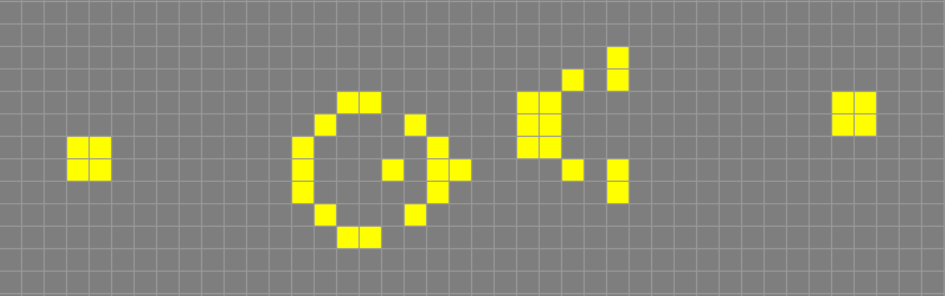
\includegraphics[width=.8\textwidth]{images/life-gosper-gun.png}
        \end{minipage}
        
        \vspace{5mm}
        El juego se hizo supremamente famoso gracias a la columna de Gardner, y gracias a la \textit{Gosper Glider gun} se pudo demostrar que el juego de la vida era un aut\'omata universal, es deicr, pod\'ia hacer cualquier c\'alculo que un computador puede hacer. El juego de la vida sigue teniendo su fanaticada incluso ahora, y todav\'ia hay una comunidad queriendo conocer m\'as sobre este.
        \vspace{7mm}
    }

    \block{Teor\'ia de juegos combinatorios}{
        Conway, Elwyn Berlekamp y Richard Guy dieron vida a \textit{Winning Ways for Your Mathematical Plays}, un compendio de cuatro vol\'umenes con toda la informaci\'on que ten\'ian sobre juegos matem\'aticos. Un trabajo que se demor\'o quince a\~nos en salir a la luz, con dos vol\'umenes, y luego en una segunda edici\'on 20 a\~nos despu\'es con dos vol\'umenes m\'as.

        En su trabajo se concentraron en generalizar el teorema de Sprague-Grundy para juegos imparciales, quer\'ian trabajar sobre juegos m\'as generales, los juegos partisanos.

        Un juego que nos permite explicar una parte de la teor\'ia de manera m\'as directa es el juego del Hackenbush.
    }
    

    
    

    \column{0.5}

    \block{}{
        

        

        \vspace{7mm}
        \innerblock{Reglas del Hackenbush}{
            El juego empieza con una configuraci\'on de l\'ineas, unas rojas y otras azules. Todas las l\'ineas tienen que estar conectadas al piso, ya sea directamente o a trav\'es de otras. El juego se juega por turnos, cada uno de los jugadores tiene un color asignado, un jugador juega con las azules y el otro juega con las rojas. En cada turno el jugador tiene que borrar una l\'inea de su color, y si alguna de las otras l\'ineas queda desconectada entonces esa tambi\'en se borra.

            \vspace{7mm}
            \begin{minipage}[t]{\linewidth}
                \centering
                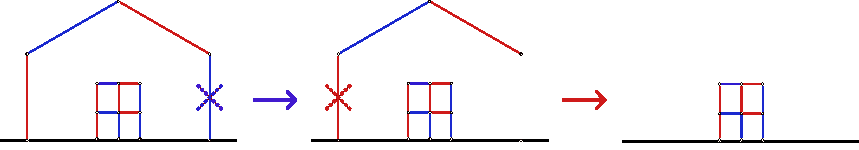
\includegraphics[width=.7\textwidth]{images/hackenbush-game_example.pdf}
            \end{minipage}
        }

        
        \vspace{5mm}
        Para la teor\'ia, a cada estado del juego se le puede asignar un valor que nos va a decir qui\'en va a ganar el juego. Si el valor es mayor a $0$ sabemos que va a ganar el azul, si es menor a $0$ va a ganar el rojo, y si es igual a $0$ entonces gana el segundo jugador. La forma en que se definen los valores es la siguiente; sea $L$ el conjunto de los valores de los estados a los que puede llegar el jugador azul, y sea $R$ el del jugador rojo, entonces el valor de nuestro estado se va a definir recursivamente como $\{L|R\}$.
        \vspace{7mm}
        
        \begin{minipage}[t]{\linewidth}
            \centering
            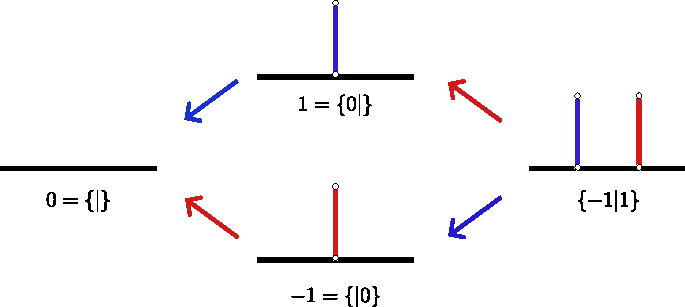
\includegraphics[width=.7\textwidth]{images/hackenbush-surr_roots.pdf}
        \end{minipage}

        Algunas configuraciones tienen ciertos `arbustos' desconectados unos de otros, por lo tanto cada uno de estos arbustos se puede tratar como un juego separado, la combinaci\'on de estos es la suma de los juegos, y el valor de este juego es la suma de los juegos separados.
        \vspace{7mm}

        \begin{minipage}[t]{\linewidth}
            \centering
            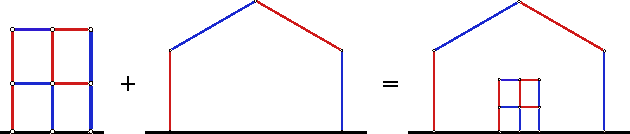
\includegraphics[width=.7\textwidth]{images/hackenbush-sum_example.pdf}
        \end{minipage}

        \vspace{5mm}
        As\'i, la suma de estos valores tiene una representaci\'on gr\'afica y queda definida como 
        \[
            x + y  \equiv \left\{x^L+y, x+y^L\;|\;x^R+y, x+y^R\right\}.
        \]
    }

    \block{N\'umeros surreales}{
        La multiplicaci\'on de valores de juegos est\'a dada por
        \[
            xy = \big\{x^Ly+xy^L-x^Ly^L, x^Ry+xy^R-x^Ry^R\big|x^Ly+xy^R-x^Ly^R, x^Ry+xy^L-x^Ry^L\big\}.
        \]

        Si tomamos la clase de valores de juegos dados por
        \[
            \mathbb{S} = \left\{\{L|R\}\;\middle|\; l\in L, r\in R, l < r\right\},
        \]
        esta clase es totalmente ordenada, adem\'as junto la suma y multiplicaci\'on definida, forman un cuerpo ordenado. A esta clase se le conoce como los n\'umeros surreales.

        Los n\'umeros surreales son una extensi\'on de los n\'umeros reales que admite infinitos e infinitesimales, adem\'as son el cuerpo ordenado m\'as grande, esto significa que todos los dem\'as cuerpos ordenados son subcuerpos de los n\'umeros surreales \cite{Bajnok2013}. Tambi\'en contienen a los ordinales.

        Conway public\'o la teor\'ia de los n\'umeros surreales en su libro \textit{On numbers and Games}\cite{Conway2000}, al principio \'el los llamaba solamente n\'umeros porque esta clase conten\'ia a todos los n\'umeros, el nombre se lo di\'o Donald Knuth en la novela \textit{Surreal Numbers}\cite{Knuth1974-wh}. Conway consideraba al descubrimiento de los n\'umeros surreales como su mejor trabajo matem\'atico.
        \vspace{5mm}

        \begin{minipage}[t]{\linewidth}
            \centering
            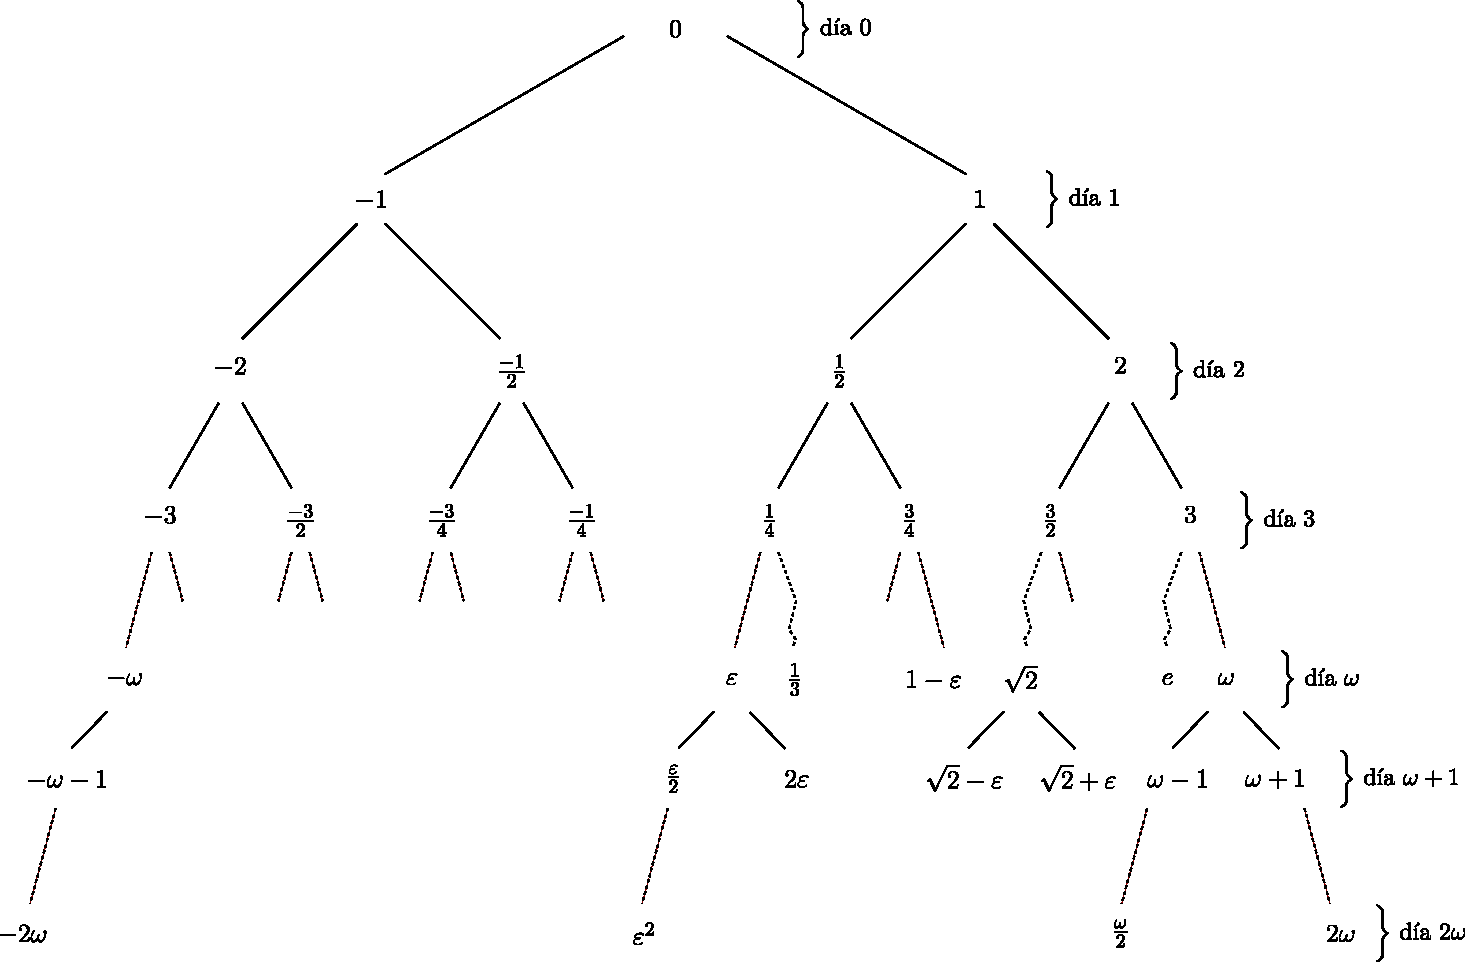
\includegraphics[width=\textwidth]{images/surreal-infinite.pdf}
        \end{minipage}
    }
    
    \block{Referencias}{
        \centering
        \printbibliography[heading=none]
    }

\end{columns}
\end{document}